\begin{figure*}[t]
    \centering
    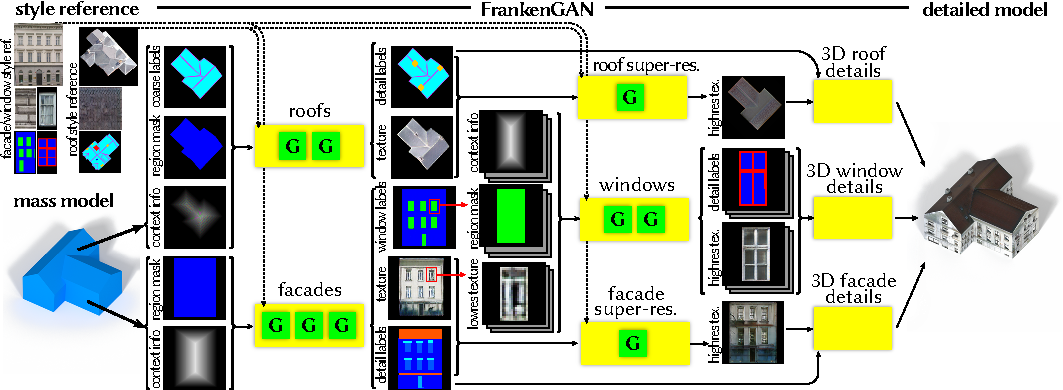
\includegraphics[width=\textwidth]{images/overview.pdf}
    \caption{\systemName overview. Individual GANs are denoted by G, and yellow rectangles denote GAN chains or geometry generation modules. Given a mass model and an optional style reference (any part can be replaced by a random style), the model is detailed in three steps. First, two chains of GANs generate texture and label maps for facades and roofs. Then, the resolution of the generated textures is increased by a dedicated window generation chain and two super-resolution GANs for roofs and facades. Finally, 3D details are generated for roofs, windows, and facades based on the generated textures and label maps.}
    \label{fig:overview}
\end{figure*}

\section{Overview}
\label{sec:overview}


The input to our method is a coarse building mass model with a given set of flat facades and a roof with known hip- and ridge-lines. Our goal is to generate texture and geometric details on the facades and the roof. These details are generated with a cascade of GANs. Our generative approach contrasts with the reconstruction performed by photogrammetric approaches, see Figure~\ref{fig:photogrammetric} for a comparison. In contrast to traditional GAN setups, our method allows control over the style of the synthesized outputs. It generates geometric detail in addition to texture detail. Geometric detail is generated by training the GANs to output an additional \emph{label map} that can be used to select the type of geometry to place at each location on the facade and roof (if any).

We interleave GANs that output structural labels with those that output textures. This leads to several desirable properties that are difficult to obtain with traditional end-to-end GAN setups:
%
Firstly, the output should exhibit a plausible structure. For example, windows tend to be arranged in grids, and the ground floor usually has a different structure than the other floors. In our experiments we found that training a GAN end-to-end makes it difficult to obtain plausible structure; the structure is never given explicitly as an objective and it must be deduced from the facade texture. The structural labels also allow us to map the output bitmaps to 3D geometry, regularize the outputs using known priors, and permit users to manually modify the structure.
%
Secondly, the user should have some control over the style of the output. Facades of the same building usually have the same style, while the amount of style variation in a block of buildings depends on the city and area. Generating realistic city blocks therefore requires control over the style. Figure~\ref{fig:photogrammetric} presents a few examples. 
%
Thirdly, we wish to improve upon the quality achievable with a generic GAN architecture like Pix2Pix~\cite{pix2pix}. While recent work has shown remarkable quality and resolution~\cite{Karras:2018:PGG}, achieving this quality with a single network trained end-to-end comes at a prohibitive resource cost.

We improve these three desirable properties in our outputs at a reasonable resource cost by splitting the traditional single-GAN setup into multiple smaller steps that can be trained and evaluated separately. Synchronization across different steps using a low-dimensional embedding of style ensures the consistency of outputs. Additionally, the style embedding can be manipulated by the user, giving control over the style distribution on a building, a block or multiple blocks.

Figure~\ref{fig:overview} shows an overview of the steps performed to generate facade and roof details. In the following, we assume that the user is working on a block of buildings, but similar steps also apply to multiple building blocks or a single building. First, the user defines style distributions for the building block. Style distributions can be provided for several building \emph{properties}, such as facade texture, roof texture, and window layouts. Each distribution is modeled as a mixture of Gaussians in a low-dimensional \emph{style space}, where the user may choose $n$ modes by providing $n$ reference images (which do not need to be consistent with the building shape or each other), and optionally a custom variance. Each building in the block samples one style vector from this distribution and uses it for all windows, facades and the roof. Specifying styles gives more control over the result, but is optional; the style for any building property can instead be entirely random. Section~\ref{sec:style_control} provides details.

After each building style is defined, two separate chains of GANs with similar architectures generate the facade and roof textures, as well as the corresponding label maps. Each GAN in the chain performs image-to-image mapping based on BicycleGAN~\cite{zhu2017multimodal}. We extend this architecture with several conditional inputs, including a mask of the empty facade or roof and several metrics describing the input, such as its approximate scale and a distance transform of the input boundary. This information about the global context makes it easier for a network that operates only on local patches to make global decisions, such as generating details at the correct scale, or placing objects such as doors at the correct height. Details about the GAN architecture are provided in Section~\ref{sec:gan_architecture}.

To generate facade textures and label maps, three of these GANs are chained together, each performing one step in the construction of the final facade details. The first GAN generates window labels from a blank facade mask; the second GAN transform these labels into the facade texture; and the final GAN detects non-window labels in the facade texture to generate a second detailed label map. Similar steps are performed for roof textures and label maps.
%Section~\ref{sec:detail_generation} provides details.
As we will show, this multi-step approach results in higher-quality details compared to an end-to-end approach.

The resolution of the facade and roof textures is limited by the memory requirements of the GANs. To obtain higher-resolution textures without significantly increasing the memory requirements, we employ two strategies: first, since windows are prominent features that usually exhibit fine details, we texture windows individually. A GAN chain creates window-pane labels in a first step and window textures from these labels in a second step. Second, we increase the resolution of the roof and wall textures using a super-resolution GAN applied to wall patches of fixed size. This GAN has the same architecture as the GANs used in all other steps. Details on all GAN chains are given in Section~\ref{sec:detail_generation}.

Finally,
3D geometric details are created based on the generated label maps using procedural geometry ,
%geometric details are lifted to 3D using procedural geometry based on the generated label maps,
and the resulting detailed mass models are textured using the generated textures.
We also use label maps and textures to define decorative 3D details and material properties maps. Details are provided in Section~\ref{sec:geometry_synthesis}. \changed{The source code and pre-trained network weights are available from the project webpage \emph{\url{http://geometry.cs.ucl.ac.uk/projects/2018/frankengan/}}.}

% single GAN
%

%Input: 3D mass models (flat facade) with dimensions + example facade images for style guidance

%Output: 2.5D geometry; still very low cost; and changeable by different facade images


%facade: blank facade > windows > texture conditioned on window labels > further labels extracted > 2,5 geometry + stylized

%Similarly, 
%roof: flat facade > straight skeleton encoding > roof slopes > textures > dormer/chimney > final textures


%style consistency: inside a floor, on a facade front; across buildings on the same street; using images as guidance
